\chapter{Protocolo de investigación}

\section{Introducción y antecedentes}
Los Algoritmos Evolutivos (Evolutionary Algorithms --- \EAS{}) son considerados como uno de los enfoques con mayor 
eficacia para resolver distintas categorías de problemas de optimización.
%
Se han desarrollado diversas variantes que han sido aplicadas en múltiples campos, como en transporte, economía o ingeniería.
%
Particularmente, se han aplicado tanto en problemas del dominio continuo (\cite{glover2005handbook}) como del 
dominio discreto (\cite{Joel:Dynamic_FAP}).
%
En general, los \EAS{} han sido especialmente exitosos en la resolución de problemas complejos en donde los enfoques exactos 
no son actualmente aplicables, como por ejemplo, en problemas NP-completos con espacios de búsqueda 
grandes (\cite{chakraborty2008advances}).
% 
\subsection{Optimizadores estocásticos poblacionales}

De acuerdo a \cite{voss2012meta}, una meta-heurística es un proceso maestro iterativo que guía y modifica un conjunto de operaciones 
heurísticas con el fin de producir de forma eficiente soluciones de calidad. 
%
Las operaciones podrían manipular una solución completa o incompleta, o incluso un conjunto de soluciones por iteración.
%
Las heurísticas subordinadas podrían ser procedimientos de alto o bajo nivel, como una búsqueda local simple, o un método 
constructivo.
%
Además, algunas de las clasificaciones bastante utilizadas en la literatura distinguen entre(\cite{beheshti2013review}):
\begin{itemize}
    \item Inspirado en la naturaleza y no-inspirado en la naturaleza.
    \item En base a la población y en base a un simple punto.
\end{itemize}

La cantidad de metaheurísticas propuestas ha crecido enormemente en los últimos años.
%
La figura \ref{fig:clasificacion} muestra algunas de las metaheurísticas más populares, clasificadas con base
en varias categorías, destacando si son o no técnicas poblacionales.
%
Este trabajo se enfoca principalmente en las meta-heurísticas poblacionales, es decir,
aquellas que consideran múltiples soluciones en cada iteración. 
%
Algunas de las metaheurísticas poblacionales más populares son las siguientes:
\begin{itemize}
	\item Algoritmos genéticos (Genetic algorithm).
	\item Programación genética (Genetic programming).
	\item Programación evolutiva (Evolutionary programming).
	\item Evolución diferencial (Differential evolution).
	\item Búsqueda dispersa (Scatter search).
	\item Estrategia evolutiva (Evolutionary strategy).
	\item Algoritmos de estimación de distribución (Estimation of distribution algorithm).
	\item Optimización por enjambre de partículas (Particle Swarm optimization).
	\item Algoritmos de optimización por colonias de hormigas (Ant colony optimization algorithms).
\end{itemize}

\begin{figure}[H]
\centering
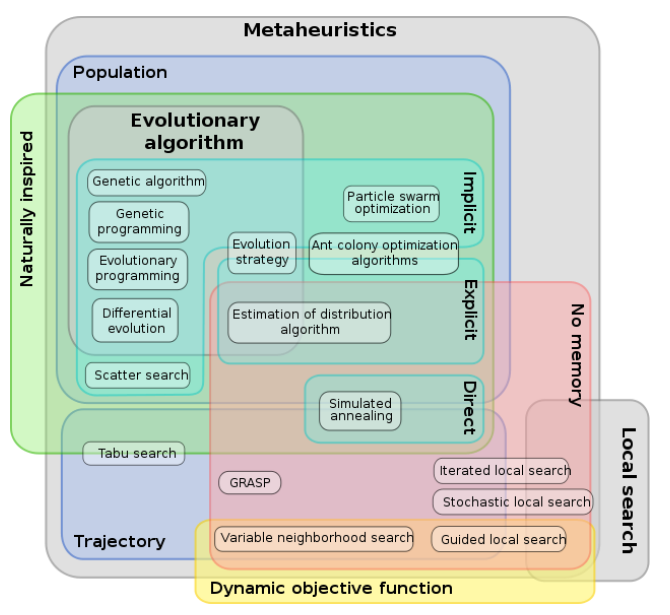
\includegraphics[width=0.8\textwidth]{clasificacion.png}
\caption{Metaheurísticas más populares con base en varios criterios de clasificación. Figura tomada de \cite{beheshti2013review}.}
\label{fig:clasificacion}
\end{figure}



\subsection{Definición del problema}

Actualmente, las metaheurísticas clasificadas como poblacionales son de las más utilizadas, especialmente
al considerar ejecuciones de largo plazo (\cite{glover2005handbook}).
%
Sin embargo, a pesar de su éxito la mayoría sufren bajo ciertas condiciones de uso problemas de convergencia acelerada
y no es fácil controlar la velocidad a la que las mismas convergen.
%
En consecuencia el proceso de búsqueda se puede estancar casi desde el inicio de su tiempo total de ejecución por lo que
se desperdiciarían recursos valiosos durante el resto de su ejecución.
%
Este problema es especialmente notorio al considerar ejecuciones de largo plazo.

\subsection{Principios de diseño de un algoritmo estocástico poblacional}

La experiencia que se ha ganado a lo largo de los años permite concluir que a la hora de diseñar 
un algoritmo evolutivo --- o de forma más general un algoritmo poblacional --- es muy importante conseguir inducir un balanceo 
adecuado entre la exploración e intensificación del espacio de búsqueda (\cite{herrera1996adaptation}).
%
Nótese en este punto que, de manera informal, la exploración del espacio de búsqueda consiste en evaluar regiones del espacio 
de búsqueda que no han sido muestreadas con el fin de detectar regiones promisorias, mientras que la explotación consiste en 
muestrear en zonas ya evaluadas previamente para realizar una búsqueda más profunda con el fin de encontrar soluciones más 
refinadas y de mayor calidad.
%
Cuando en los algoritmos poblacionales todas o casi todas las soluciones están en regiones distantes --- alta diversidad --- se 
produce habitualmente una búsqueda exploratoria, es decir, muchas de las nuevas soluciones evaluadas serán distantes a las ya 
evaluadas anteriormente.
%
Sin embargo, cuando casi todas las soluciones están en una o en unas pocas regiones, se suele producir 
una búsqueda intensificadora.
%
Uno de los problemas en el diseño de los algoritmos evolutivos y otros esquemas poblacionales es que en muchos casos no se 
comprenden todas las implicaciones que los diferentes componentes tienen sobre el mantenimiento de la diversidad de la población 
y en consecuencia sobre el balanceo entre exploración e intensificación (\cite{Crepinsek:13}).
%
Por ello, analizar el comportamiento y rediseñar con base en lo que está ocurriendo en este aspecto, es parte del proceso de 
diseño de los algoritmos evolutivos.

Relacionado con lo anterior, aparece el concepto de convergencia prematura (\cite{Crepinsek:13}).
%
Se dice que un algoritmo converge de forma prematura cuando mucho antes de alcanzar el criterio de paro, todas las soluciones 
están en una zona muy pequeña del espacio de búsqueda.
%
En este sentido, a partir de ese momento es difícil seguir mejorando las soluciones de forma significativa ya que con alta 
probabilidad sólo se va a realizar un muestreo de soluciones en dicha región.
%
Por ello, es importante detectar si esto ocurre y en tal caso rediseñar algunos aspectos del algoritmo para preservar una i
mayor diversidad.
%
Sin embargo, si la población es muy diversa durante todo el proceso de búsqueda, se podría no alcanzar un grado adecuado de 
intensificación y por lo tanto se tendría una convergencia lenta que posiblemente también resultaría en soluciones de baja calidad.

\subsection{Importancia de la diversidad, criterio de parada y tiempo transcurrido en optimización combinatoria}

En los últimos años, algunos de los trabajos más exitosos en el área de optimización combinatoria mono-objetivo han incluido
mecanismos para gestionar diversidad de forma explícita en el espacio de las variables considerando para ello el tiempo transcurrido 
y el criterio de parada.
%
Este tipo de métodos han encontrado los mejores resultados en varios problemas de optimización combinatoria, como es el problema 
de asignación de frecuencias \citetitle{Joel:Dynamic_FAP} (\cite{Joel:Dynamic_FAP}), el problema del Sudoku 
\citetitle{Joel:Dynamic_Sudoku} (\cite{Joel:Dynamic_Sudoku}), el problema del agente viajero 
\citetitle{Joel:ANovelDiversityBasedEAForTheTSP} (\cite{Joel:ANovelDiversityBasedEAForTheTSP}),
el problema de particionado de grafos \citetitle{romero2018memetic} (\cite{romero2018memetic}), 
o el problema de embalaje bidimensional \citetitle{segredo2014memetic} (\cite{segredo2014memetic}).
%
Por ello, se puede concluir que en dicha área, rediseñar las componentes de los algoritmos evolutivos tomando decisiones con base
en la diversidad, criterio de parada y tiempo o generaciones transcurridos es de vital importancia.
